%%Copyright 2021. Any replication of this document is permissible. The primary package of this document is from cjquines%%

%%PRIMARY PREAMBLE%%
\documentclass[11pt,paper=letter]{scrartcl}
\usepackage[ boxthm, parskip]{cjquines}
\usepackage{CJKutf8}
\usepackage{jrobaob}



\begin{document}


\title{Week 1 Random Problems}
\author{\joshbluebf{Problems of the Week — Season 3}}
\date{March 18, 2022}

\maketitle
\setlength{\unitlength}{1in}
\begin{picture}(2,0)
  \put(1.20,1.35){\hbox{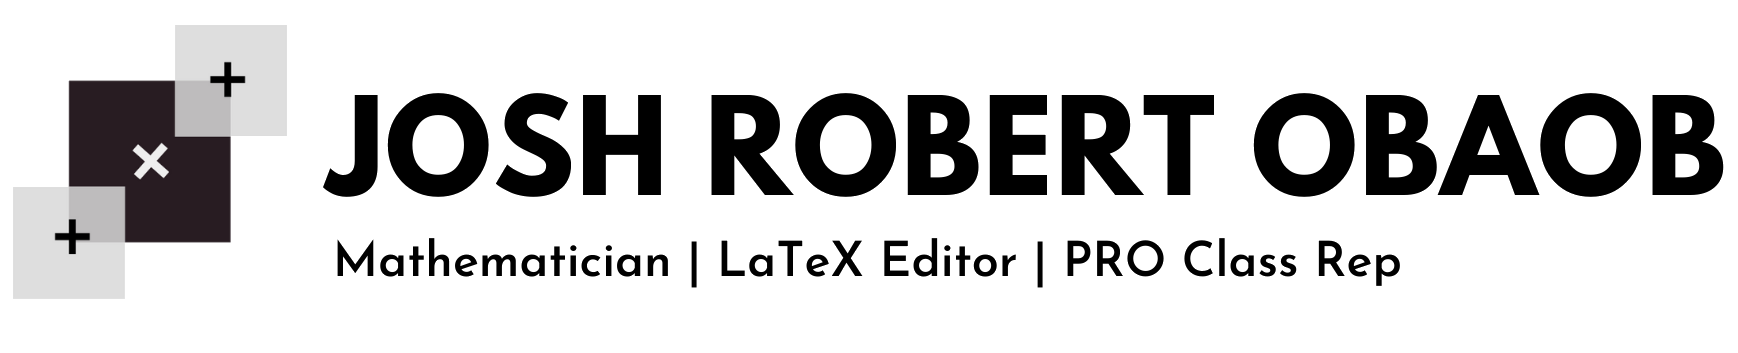
\includegraphics[width=4.2in]{logo2.png}}}
\end{picture}
\vspace{-2em}


\begin{abstract}
Hello there! This is the first episode of the new season of my mathematical series, \joshbf{Problems of the Week}. After weeks of experiencing the \textit{avalanche} of school works, somehow, I can finally resume the posting of my series with a \joshbluebf{new season.} 
\end{abstract}

\vspace{-2em}

\section{Problems}

\probn1  In triangle $ABC$, let $D$ be the point on the opposite side of line $BC$ as $A$ such that $\overline{AB} \parallel \overline{CD}$. Given that $AB=BD=8$, $BC=9$, and $CD=4$, what is $AD^2$?

\begin{center}
    


\tikzset{every picture/.style={line width=0.75pt}} %set default line width to 0.75pt        

\begin{tikzpicture}[x=0.75pt,y=0.75pt,yscale=-1,xscale=1]
%uncomment if require: \path (0,396); %set diagram left start at 0, and has height of 396

%Shape: Triangle [id:dp8774143694309666] 
\draw   (195.8,68) -- (290.8,182) -- (140,182) -- cycle ;
%Straight Lines [id:da1158230916152363] 
\draw  [dash pattern={on 4.5pt off 4.5pt}]  (195.8,68) -- (262.8,240) ;
\draw [shift={(262.8,240)}, rotate = 68.72] [color={rgb, 255:red, 0; green, 0; blue, 0 }  ][fill={rgb, 255:red, 0; green, 0; blue, 0 }  ][line width=0.75]      (0, 0) circle [x radius= 2.01, y radius= 2.01]   ;
\draw [shift={(195.8,68)}, rotate = 68.72] [color={rgb, 255:red, 0; green, 0; blue, 0 }  ][fill={rgb, 255:red, 0; green, 0; blue, 0 }  ][line width=0.75]      (0, 0) circle [x radius= 2.01, y radius= 2.01]   ;
%Straight Lines [id:da5172000492574442] 
\draw  [dash pattern={on 4.5pt off 4.5pt}]  (140,182) -- (262.8,240) ;
\draw [shift={(140,182)}, rotate = 25.28] [color={rgb, 255:red, 0; green, 0; blue, 0 }  ][fill={rgb, 255:red, 0; green, 0; blue, 0 }  ][line width=0.75]      (0, 0) circle [x radius= 2.01, y radius= 2.01]   ;
%Straight Lines [id:da36853724749820493] 
\draw  [dash pattern={on 4.5pt off 4.5pt}]  (290.8,182) -- (262.8,240) ;
\draw [shift={(290.8,182)}, rotate = 115.77] [color={rgb, 255:red, 0; green, 0; blue, 0 }  ][fill={rgb, 255:red, 0; green, 0; blue, 0 }  ][line width=0.75]      (0, 0) circle [x radius= 2.01, y radius= 2.01]   ;

% Text Node
\draw (196.72,50.53) node    {$A$};
% Text Node
\draw (128.39,182.2) node    {$B$};
% Text Node
\draw (304.72,182.53) node    {$C$};
% Text Node
\draw (263.05,257.53) node    {$D$};


\end{tikzpicture}
\end{center}


\probn2 Suppose an equation $$\dfrac{A}{162x^2 +99x + 14} + \dfrac{B}{405x^2 +153x + 14} = \dfrac{C}{810x^2 +441x + 49}.$$ Find all ordered triples $(A,B,C)$ such that $\text{gcd}(A, B, C)=1$. 

\probn3 Let ${a_n}$ defined at $n \geq 1$ be a sequence of rational numbers. This sequence begins with $a_1= 1$, then continues, with the next, succeeding terms satisfying $a_1 + 2a_2 + 3a_3 + 4a_4 + ... + n(a_n) = (n + 1)a_{n + 1}$. For some positive integer $k$, $$ \sum_{n=1}^{k} \dfrac{3a_{3n}}{a_n \cdot a_{2n}} = 19316.$$ Find the numerical value of $k$.


\vspace{2cm}

\newpage

\section{Solutions}

\subsection{Problem 1}

\vspace{2mm}


\begin{mdframed}[style=jremmdbox, frametitle = Problem 1]

 In triangle $ABC$, let $D$ be the point on the opposite side of line $BC$ as $A$ such that $\overline{AB} \parallel \overline{CD}$. Given that $AB=BD=8$, $BC=9$, and $CD=4$, what is $AD^2$?

\begin{center}
    


\tikzset{every picture/.style={line width=0.75pt}} %set default line width to 0.75pt        

\begin{tikzpicture}[x=0.75pt,y=0.75pt,yscale=-1,xscale=1]
%uncomment if require: \path (0,396); %set diagram left start at 0, and has height of 396

%Shape: Triangle [id:dp8774143694309666] 
\draw   (195.8,68) -- (290.8,182) -- (140,182) -- cycle ;
%Straight Lines [id:da1158230916152363] 
\draw  [dash pattern={on 4.5pt off 4.5pt}]  (195.8,68) -- (262.8,240) ;
\draw [shift={(262.8,240)}, rotate = 68.72] [color={rgb, 255:red, 0; green, 0; blue, 0 }  ][fill={rgb, 255:red, 0; green, 0; blue, 0 }  ][line width=0.75]      (0, 0) circle [x radius= 2.01, y radius= 2.01]   ;
\draw [shift={(195.8,68)}, rotate = 68.72] [color={rgb, 255:red, 0; green, 0; blue, 0 }  ][fill={rgb, 255:red, 0; green, 0; blue, 0 }  ][line width=0.75]      (0, 0) circle [x radius= 2.01, y radius= 2.01]   ;
%Straight Lines [id:da5172000492574442] 
\draw  [dash pattern={on 4.5pt off 4.5pt}]  (140,182) -- (262.8,240) ;
\draw [shift={(140,182)}, rotate = 25.28] [color={rgb, 255:red, 0; green, 0; blue, 0 }  ][fill={rgb, 255:red, 0; green, 0; blue, 0 }  ][line width=0.75]      (0, 0) circle [x radius= 2.01, y radius= 2.01]   ;
%Straight Lines [id:da36853724749820493] 
\draw  [dash pattern={on 4.5pt off 4.5pt}]  (290.8,182) -- (262.8,240) ;
\draw [shift={(290.8,182)}, rotate = 115.77] [color={rgb, 255:red, 0; green, 0; blue, 0 }  ][fill={rgb, 255:red, 0; green, 0; blue, 0 }  ][line width=0.75]      (0, 0) circle [x radius= 2.01, y radius= 2.01]   ;

% Text Node
\draw (196.72,50.53) node    {$A$};
% Text Node
\draw (128.39,182.2) node    {$B$};
% Text Node
\draw (304.72,182.53) node    {$C$};
% Text Node
\draw (263.05,257.53) node    {$D$};


\end{tikzpicture}
\end{center}
\end{mdframed}

\ans{$AD^2 = 128.$}

\soln1 From the given fact that $AB \parallel CD$, $ACBD$ is a trapezoid. Draw an auxiliary line from $C$ to a point $N$ on $AB$ such that $CD \parallel NB,$ making $NB = \frac{1}{2}AB$.

\begin{center}
    


\tikzset{every picture/.style={line width=0.75pt}} %set default line width to 0.75pt        

\begin{tikzpicture}[x=0.75pt,y=0.75pt,yscale=-1,xscale=1]
%uncomment if require: \path (0,396); %set diagram left start at 0, and has height of 396

%Shape: Triangle [id:dp8774143694309666] 
\draw   (195.8,68) -- (290.8,182) -- (140,182) -- cycle ;
%Straight Lines [id:da1158230916152363] 
\draw  [dash pattern={on 4.5pt off 4.5pt}]  (195.8,68) -- (262.8,240) ;
\draw [shift={(262.8,240)}, rotate = 68.72] [color={rgb, 255:red, 0; green, 0; blue, 0 }  ][fill={rgb, 255:red, 0; green, 0; blue, 0 }  ][line width=0.75]      (0, 0) circle [x radius= 2.01, y radius= 2.01]   ;
\draw [shift={(195.8,68)}, rotate = 68.72] [color={rgb, 255:red, 0; green, 0; blue, 0 }  ][fill={rgb, 255:red, 0; green, 0; blue, 0 }  ][line width=0.75]      (0, 0) circle [x radius= 2.01, y radius= 2.01]   ;
%Straight Lines [id:da5172000492574442] 
\draw  [dash pattern={on 4.5pt off 4.5pt}]  (140,182) -- (262.8,240) ;
\draw [shift={(140,182)}, rotate = 25.28] [color={rgb, 255:red, 0; green, 0; blue, 0 }  ][fill={rgb, 255:red, 0; green, 0; blue, 0 }  ][line width=0.75]      (0, 0) circle [x radius= 2.01, y radius= 2.01]   ;
%Straight Lines [id:da36853724749820493] 
\draw  [dash pattern={on 4.5pt off 4.5pt}]  (290.8,182) -- (262.8,240) ;
\draw [shift={(290.8,182)}, rotate = 115.77] [color={rgb, 255:red, 0; green, 0; blue, 0 }  ][fill={rgb, 255:red, 0; green, 0; blue, 0 }  ][line width=0.75]      (0, 0) circle [x radius= 2.01, y radius= 2.01]   ;
%Straight Lines [id:da8236690754502436] 
\draw [color={rgb, 255:red, 137; green, 22; blue, 22 }  ,draw opacity=1 ] [dash pattern={on 4.5pt off 4.5pt}]  (167.9,125) -- (290.7,183) ;
\draw [shift={(167.9,125)}, rotate = 25.28] [color={rgb, 255:red, 137; green, 22; blue, 22 }  ,draw opacity=1 ][fill={rgb, 255:red, 137; green, 22; blue, 22 }  ,fill opacity=1 ][line width=0.75]      (0, 0) circle [x radius= 2.01, y radius= 2.01]   ;

% Text Node
\draw (196.72,50.53) node    {$A$};
% Text Node
\draw (128.39,182.2) node    {$B$};
% Text Node
\draw (304.72,182.53) node    {$C$};
% Text Node
\draw (263.05,257.53) node    {$D$};
% Text Node
\draw (154.72,115.53) node    {$N$};


\end{tikzpicture}
\end{center}

and $NC \parallel BD$. This implies that $NC$ is the altitude of the trapezoid and $BD = NC = 8$, making $NCBD$ a rectangle. Hence, \fbox{$AD^2 = 128.$}

\newpage

\soln2 Extend $CD$ to point $A'$ such that $AA' \perp AB$, making $AD$ a diagonal of the quadrilateral $AA'BD$.

\begin{center}
    


\tikzset{every picture/.style={line width=0.75pt}} %set default line width to 0.75pt        

\begin{tikzpicture}[x=0.75pt,y=0.75pt,yscale=-1,xscale=1]
%uncomment if require: \path (0,396); %set diagram left start at 0, and has height of 396

%Shape: Triangle [id:dp4989487816040732] 
\draw   (384.6,71.2) -- (479.6,185.2) -- (328.8,185.2) -- cycle ;
%Straight Lines [id:da09874329017898242] 
\draw  [dash pattern={on 4.5pt off 4.5pt}]  (384.6,71.2) -- (451.6,243.2) ;
\draw [shift={(451.6,243.2)}, rotate = 68.72] [color={rgb, 255:red, 0; green, 0; blue, 0 }  ][fill={rgb, 255:red, 0; green, 0; blue, 0 }  ][line width=0.75]      (0, 0) circle [x radius= 2.01, y radius= 2.01]   ;
\draw [shift={(384.6,71.2)}, rotate = 68.72] [color={rgb, 255:red, 0; green, 0; blue, 0 }  ][fill={rgb, 255:red, 0; green, 0; blue, 0 }  ][line width=0.75]      (0, 0) circle [x radius= 2.01, y radius= 2.01]   ;
%Straight Lines [id:da8508938249000904] 
\draw  [dash pattern={on 4.5pt off 4.5pt}]  (328.8,185.2) -- (451.6,243.2) ;
\draw [shift={(328.8,185.2)}, rotate = 25.28] [color={rgb, 255:red, 0; green, 0; blue, 0 }  ][fill={rgb, 255:red, 0; green, 0; blue, 0 }  ][line width=0.75]      (0, 0) circle [x radius= 2.01, y radius= 2.01]   ;
%Straight Lines [id:da9437598218379355] 
\draw  [dash pattern={on 4.5pt off 4.5pt}]  (479.6,185.2) -- (451.6,243.2) ;
\draw [shift={(479.6,185.2)}, rotate = 115.77] [color={rgb, 255:red, 0; green, 0; blue, 0 }  ][fill={rgb, 255:red, 0; green, 0; blue, 0 }  ][line width=0.75]      (0, 0) circle [x radius= 2.01, y radius= 2.01]   ;
%Straight Lines [id:da6501116222419803] 
\draw [color={rgb, 255:red, 137; green, 22; blue, 22 }  ,draw opacity=1 ] [dash pattern={on 4.5pt off 4.5pt}]  (507.4,129.2) -- (479.6,185.2) ;
\draw [shift={(507.4,129.2)}, rotate = 116.4] [color={rgb, 255:red, 137; green, 22; blue, 22 }  ,draw opacity=1 ][fill={rgb, 255:red, 137; green, 22; blue, 22 }  ,fill opacity=1 ][line width=0.75]      (0, 0) circle [x radius= 2.01, y radius= 2.01]   ;
%Straight Lines [id:da0843026287077453] 
\draw [color={rgb, 255:red, 65; green, 117; blue, 5 }  ,draw opacity=1 ] [dash pattern={on 4.5pt off 4.5pt}]  (384.6,71.2) -- (507.4,129.2) ;
\draw [shift={(384.6,71.2)}, rotate = 25.28] [color={rgb, 255:red, 65; green, 117; blue, 5 }  ,draw opacity=1 ][fill={rgb, 255:red, 65; green, 117; blue, 5 }  ,fill opacity=1 ][line width=0.75]      (0, 0) circle [x radius= 2.01, y radius= 2.01]   ;

% Text Node
\draw (385.52,53.73) node    {$A$};
% Text Node
\draw (317.19,185.4) node    {$B$};
% Text Node
\draw (493.52,185.73) node    {$C$};
% Text Node
\draw (451.85,260.73) node    {$D$};
% Text Node
\draw (343.52,118.73) node    {$N$};


\end{tikzpicture}
\end{center}

Since $AA' \perp AB$, then $AD^2 = AB^2 + BD^2 = 128.$


\subsection{Problem 2}

\vspace{2mm}



\begin{mdframed}[style=jremmdbox, frametitle = Problem 2]
Suppose an equation $$\dfrac{A}{162x^2 +99x + 14} + \dfrac{B}{405x^2 +153x + 14} = \dfrac{C}{810x^2 +441x + 49}.$$ Find all ordered triples $(A,B,C)$ such that $\text{gcd}(A, B, C)=1$. 
\end{mdframed}

\ans{$(1,1,7)$}

\sol The equation can be rewritten into $$\dfrac{A}{(18x +7)(9x+2)} + \dfrac{B}{(45x+7)(9x+2)} = \dfrac{C}{(45x +7)(18x+7)}.$$ Notice that the LCM of the denominators is $(18x+7)(45x+7)(9x+2)$ and therefore, $$\dfrac{A(45x+7) + B(18x+7)}{(18x +7)(9x+2)(45x+7)}  = \dfrac{C}{(45x +7)(18x+7)}.$$ But since the denominator at the right hand side of the equation has no $(9x +2)$, then $A(45x+7) + B(18x+7)$ must be a multiple of $9x+2$. 

By observing the equation, we see that $A=B=1$, making $C = 7$. Hence, our triple is \fbox{$(A,B,C) = (1,1,7)$.}

\newpage

\subsection{Problem 3}

\vspace{2mm}



\begin{mdframed}[style=jremmdbox, frametitle = Problem 3]
Let ${a_n}$ defined at $n \geq 1$ be a sequence of rational numbers. This sequence begins with $a_1= 1$, then continues, with the next, succeeding terms satisfying $a_1 + 2a_2 + 3a_3 + 4a_4 + ... + n(a_n) = (n + 1)a_{n + 1}$. For some positive integer $k$, $$ \sum_{n=1}^{k} \dfrac{3a_{3n}}{a_n \cdot a_{2n}} = 19316.$$ Find the numerical value of $k$.
\end{mdframed}

\ans {69}

\sol Let us do some evaluation:

\begin{itemize}
    \item If $n=1$, then $a_2 = 1/2$
    \item If $n=2$, then $a_3 = 2/3$
    \item If $n=3$, then $a_4 = 1$
    
\end{itemize}

By engineering, $a_n = \frac{2^{n}}{4n}$ for all $n \geq 2.$ Then, the summation can be rewritten as $$\sum_{n=1}^k \dfrac{3a_{3n}}{a_n \cdot a_{2n}} = \sum_{n=1}^k \dfrac{3 \cdot \frac{2^{3n}}{12n}}{\frac{2^{2n}}{8n} \cdot \frac{2^n}{4n}} \implies \sum_{n=1}^k 8n = 19316 $$ But notice that that the first term of the summation which is $\frac{3a_{3}}{a_1 \cdot a_{2}}$ \footnote{Denote each term as $b_n = \frac{3a_{3n}}{a_n \cdot a_{2n}}$} does not satisfy to the equation (when $a_n$ generates) because $b_1 = 4.$ Hence, we add 4 to 19316 for it to become a summation of $8n$ from $n = 1$ to $k.$

Hence, we have $4k(k+1) = 19320$ and finding $k$ gives us \fbox{69.}

\vspace{2cm}

\emph{(The document is created for my deceased grandmother, Lola Rosa Bardiago Obaob. May her soul rest in peace.)}

\begin{center}

\includegraphics[width=3in]{JOSH ROBERT OBAOB (2).png}
\end{center}



\end{document}
